\documentclass[11pt,a4paper]{article}
\title{APG4011F Assignment 2 Report}
\date{21 April 2015}
\author{Tim Marsh}

\usepackage{amsmath}
\usepackage{graphicx}
\usepackage{float}
\usepackage{textcomp}
\usepackage{siunitx}
\usepackage{wrapfig}
\usepackage{caption}
\usepackage{subcaption}

\usepackage[margin=1in]{geometry}

\graphicspath{ {./} }
\begin{document}
	
	\pagenumbering{gobble}
	\maketitle
	\begin{figure}[H]
		\centering
		
\includegraphics[width=0.7\linewidth]{./UCTcircular_logo1_CMYK}
		\label{fig:UCTcircular_logo1_CMYK}
	\end{figure}
	\newpage
	\pagenumbering{arabic}
	\tableofcontents
	\listoffigures
	\newpage
	
	
	\section{Introduction}
	
	There are three parts to this assignment:
	
	\begin{description}
			\item[1. Simulating a camera, image points and object points] Creating the Cameras with made up parameters, $Xo$, $Yo$, $Zo$, $\kappa$, $\phi$, $\omega$. Creating 30 image points and calculating the corresponding ground coordinates for those image points.
			
			\item[2. Intersection] After creating a new camera, with its own orientation parameters, calculate the corresponding image point coordinates.
			
			Then using least squares calculate the best fit ground coordinates for both images.
			
			\item[3. Resection] Using the object coordinates from part 1 along with the corresponding image points, set up a least squares solution solution to determine the exterior orientation parameters of the image. do this for both images
			
			\item[4. Bundle adjustment] Treat 25 of the 30 points as control points and the remaining 5 as tie points. Use the collinearity equations to setup a least squares solution to simultaneously determine the exterior orientation parameters of the two images and the object coordinates of the tie points.
			
	\end{description}
	
	These 4 parts are done as one single program written in python that runs from start to finish. the first two cameras are defined with orientation parameters, object points and image points. Each time some action needs to be preformed on a camera a new camera instance is created and the things that need to be calculated are cleared, calculated and saved in the new instance so that they can be compared to the original values.
	
	\section{Program structure}
	
	im order to store a lot of information in a program without losing any, and being able to access it whenever is necessary. This is done with dictionaries within dictionaries.
	
	The main dictionary is Cameras, Cameras holds the image size as well as the focal length of the camera (the focal length is constant through all images). in the Cameras dictionary are Images there are multiple images (in this case 2) the Images class holds the exterior orientation parameters of that Image(photograph).
	
	Each image has image points and object points, to keep the image points and object points paired up in created and saved them in a ray class. It holds no information other than keeping the image and object points paired up.
	
	Figure 1 shows a very basic representation of the structure.
	
	\begin{figure}[H]
		\centering
		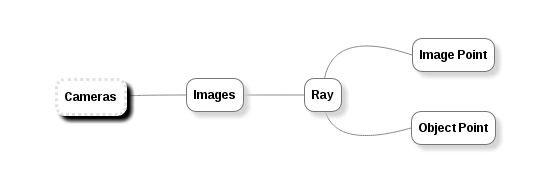
\includegraphics[width=0.7\linewidth]{/images/crop}
		\caption{Structure of Dictionaries}
		\label{fig:structure}
	\end{figure}


	\section{Background to the Problem}
	
	Knowledge of how photogrammetry works is necessary for this assignment. Each image has its image center $Xo$ $Yo$ $Zo$ as well as rotations around the $x$ $y$ and $z$ axes, $\kappa$ $\phi$ $\omega$. 
	
	\section{Method}
	
	In the first part ground coordinates are calculated using the collinearity equations. the basic form of the collinearity equations take object points or image points and calculates the other.\\
	\\
	
	$
	\centering
	\begin{bmatrix}
		X - Xo \\ 
		Y - Yo \\ 
		Z - Zo
	\end{bmatrix}= kR^T$
	$
	\begin{bmatrix}
		y \\ 
		x \\ 
		-c
	\end{bmatrix}
	$
	where R = $R\kappa R\phi R\omega$ and $k$ = scale\\
	\\
	
	In the second part this formula is reversed so that image coordinates are being calculated from the object points calculated in part 1.
	
	These are easy steps and involve going through each point in the images and calculating its corresponding point in either the image or object space. Part 3 and 4 are more complex and involve least squares to solve.\\
	
	Part 3 consists of calculating the exterior orientation parameters for an image having only image and object points. this is done through least squares. 
	
	There are 6 unknowns; $Xo$, $Yo$, $Zo$, $\kappa$, $\phi$, $\omega$ as well as a scale ($k$) for each point. This means that for every point you add in one more unknown must be added. Each point brings 2 equations so there needs to be a minimum of 5 points to solve the single bundle adjustment. this is no problem because we have 30.\\
	
	In part 4 we have a similar problem except that we don't know the object coordinates. so in order to solve this we need to use 2 images simultaneously. of our 30 points we have 25 control points and 5 tie points.
	
	
	\section{Results}
	
	The results of this are hard to showcase with out some graphical representation.
	
	
\begin{figure}[H]
\centering
\includegraphics[width=0.7\linewidth]{"/images/one image"}
\caption{}
\label{fig:oneimage}
\end{figure}
	
\begin{figure}[H]
\centering
\includegraphics[width=0.7\linewidth]{"/images/two images"}
\caption{}
\label{fig:twoimages}
\end{figure}

	
\end{document}	